\chapter{Revue de littérature sur la tâche d'annotation en intelligence artificielle}
\label{chapter:2-REVUE-DE-LITTERATURE}
	\todo[inline]{CHAPITRE: TITRE À TROUVER: "\textit{(Revue de littérature)}"}
	
	% RÉSUMÉ DES ÉPISODES PRÉCÉDENTS: 
	\todo[inline]{CHAPITRE: INTRODUCTION À RÉDIGER}
	
	% ANNONCE DU BUT DU CHAPITRE: 
	\todo[inline]{CHAPITRE: INTRODUCTION À RÉDIGER}
	
	% TABLE DES MATIÈRES DU CHAPITRE
    \minitoc
	
    %%%%%--------------------------------------------------------------------
    %%%%% Section 2.1:
    %%%%%--------------------------------------------------------------------
    \section{Présentation théorique de l'annotation}
	\label{section:2.1-PRESENTATION-ANNOTATION}
	
		% Introduction: donner une définition de ce qu'est l'annotation.
		Tout d'abord, définissons ce que nous appelons « \texttt{annotation} » et donnons quelques exemples pour comprendre les enjeux qui y sont associés.
		
		
		%%%
		%%% Subsection 2.1.1: Définition et objectifs de l'annotation de données.
		%%%
		\subsection{Définition et objectifs de l'annotation de données}
		\label{section:2.1.1-PRESENTATION-ANNOTATION-DEFINITION}
			
			%%% Corpus.
			\paragraph{Qu'est qu'un « \texttt{corpus} » ?}
			% Définition de "corpus".
			Certains phénomènes peuvent être difficiles à cerner à cause de leur nature complexe : c'est le cas par exemple avec le langage humain, la diversité de la faune et de la flore, les variétés d'un répertoire musical ou cinématographique, ...
			Pour nous aider à capturer ces phénomène et à mieux les comprendre, il est possible de les décrire par l'exemple en recueillant des textes, des images, des sons, des vidéos, ou tout autres relevés d'informations : nous utilisons alors le terme « \textbf{corpus} » pour désigner cet ensemble de données.
			Par aspect pratique, il est généralement stocké dans un format exploitable par une machine (\textit{fichier texte, base de données, ...}).
			
			% Carcatéristique importante : la représentativité !
			Un corpus n'est qu'un échantillon de taille finie d'un phénomène pouvant être infini ou indénombrable.
			Il est donc d'usage de valoriser un corpus s'il est « \textbf{représentatif} » du phénomène qu'il décrit, c'est-à-dire s'il capture bien le large panel de variations que peuvent prendre les données (\cite{biber:1993:representativeness-corpus-design}).
			
			% References.
			\begin{leftBarInformation}
				Si vous voulez mieux comprendre cette notion de corpus, vous pouvez vous référer à \cite{sinclair:2004:corpus-text-basic} issu du livre \textit{Developing Linguistic Corpora} (\cite{wynne:2004:developing-linguistic-corpora}).
			\end{leftBarInformation}
			
			%%% Annotation.
			\paragraph{Qu'est que l'« \texttt{annotation} » ?}
			% Définition de "annotation".
			Les données d'un corpus manquent parfois d'information pour bien cerner un phénomène, il est alors nécessaire de faire intervenir un humain pour introduire des connaissances supplémentaires qui ne sont pas explicitement présentes dans les données.
			Nous appelons alors « \texttt{annotation} » cette tâche consistant à décrire les données d'un corpus.
			On distingue alors les données dites « \textbf{brutes} » des données dites « \textbf{annotées} » en fonction de l'absence ou la présence d'un complément d'informations.
			
			% Valeurs associées: valeur ajoutée, information d'interprétation.
			Dans la littérature, \cite{garside-etal:1997:corpus-annotation-linguistic} présente l'annotation comme la tâche permettant de donner une « \textbf{valeur ajoutée} » aux données ; de son côté, \cite{leech:2004:adding-linguistic-annotation} précise que l'annotation permet ainsi d'interpréter les données pour mieux comprendre un phénomène, mais aussi d'entraîner un modèle d'apprentissage automatique pour le prédire voire le reproduire.
		
		
		%%%
		%%% Subsection 2.1.2: Exemples de tâches d'annotations.
		%%%
		\subsection{Exemples de tâches d'annotations}
		\label{section:2.1.2-PRESENTATION-ANNOTATION-EXEMPLES}
			
			% Transition: définitions assez généralistes car champ d'application très vaste.
			Les définitions données dans la \textsc{Section~\ref{section:2.1.1-PRESENTATION-ANNOTATION-DEFINITION}} sont volontairement assez générales car il est difficile de
			dépeindre la vaste diversité d'applications faisant intervenir de l'annotation.
			Pour mieux dresser le portrait de cette tâche, nous proposons de présenter quelques exemples sur différents cas d'usages.
			
			% Exemples données tabulaire: régression linéaire d'un prix, d'une surface, ...
			\paragraph{Exemples d'annotations de données tabulaires.}
				Certaines catégories de problèmes sont 
				\todo[inline]{SECTION: À RÉDIGER}
			
			% Exemples images: classification de document, catégorisation, détection d'objets, ...
			\paragraph{Exemples d'annotations d'images.}
				
				\todo[inline]{SECTION: À RÉDIGER}
				
				\begin{leftBarExamples}
					Annotation d'une reconnaissance optique de caractères (\texttt{OCR}) sur une image (\textsc{Figure~\ref{figure:2.1.2-PRESENTATION-ANNOTATION-EXEMPLES-IMAGE-OCR}}).
					\begin{figure}[H]
						\centering
						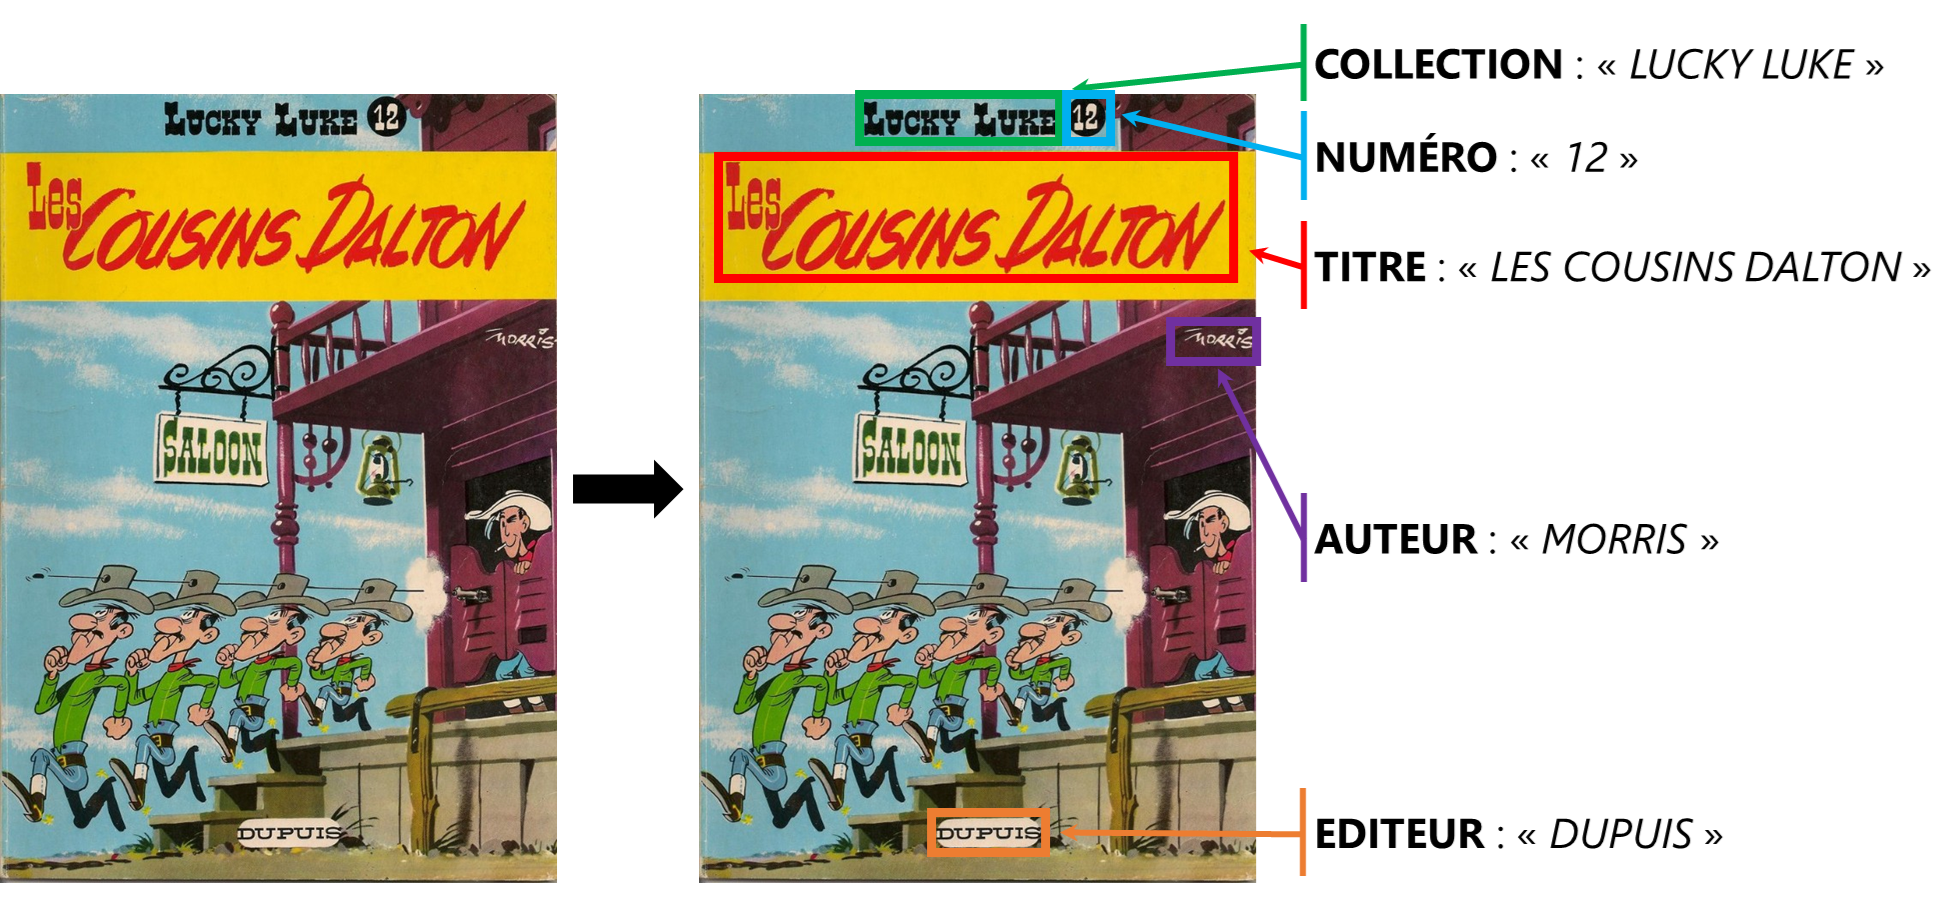
\includegraphics[width=0.95\textwidth]{figures/etatdelart-morris-1958-lucky-luke-12}
						\caption{
							Exemple d'annotation de textes présents dans une image, exemple réalisé sur la couverture de \texttt{BD} (\cite{morris-goscinny:1958:cousins-dalton}).
						}
						\label{figure:2.1.2-PRESENTATION-ANNOTATION-EXEMPLES-IMAGE-OCR}
					\end{figure}
				\end{leftBarExamples}
			
			% Exemples audio: transcription de la parole, classification de sentiment, extraction de séquence, ...
			\paragraph{Exemples d'annotations d'audios.}
				\todo[inline]{SECTION: À RÉDIGER}
			
			% Exemples textes: catégorisation, détection de sentiment, extraction d'entités nommées, ...
			\paragraph{Exemples d'annotations de textes.}
				\todo[inline]{SECTION: À RÉDIGER}
				
				\begin{leftBarExamples}
					Annotation d'une classification de textes suivant leur langue.
					\begin{quote}
						« \textit{
							Je m'appelle Erwan.
						} » \texttt{Français} \\
						« \textit{
							My name is Erwan.
						} » \texttt{Anglais} \\
						« \textit{
							Ich hei{\ss}e Erwan.
						} » \texttt{Français}
					\end{quote}
				\end{leftBarExamples}
				
				\begin{leftBarExamples}
					Annotation d'entités nommés dans un texte.
					\begin{quote}
						« \textit{
							$\textbf{\text{Erwan}}_{\texttt{(personne)}}$, un $\textbf{\text{alsacien}}_{\texttt{(origine)}}$ né en $\textbf{\text{02/09/1995}}_{\texttt{(date)}}$, réalise sa thèse avec le $\textbf{\text{LORIA}}_{\texttt{(organisation)}}$ et $\textbf{\text{Euro Information}}_{\texttt{(organisation)}}$.
						} »
					\end{quote}
				\end{leftBarExamples}
				
				\begin{leftBarExamples}
					Annotation des étiquettes grammaticales dans un texte.
					\begin{quote}
						« \textit{
							$\text{Hier}_{\texttt{(ADV)}}$,
							$\text{Erwan}_{\texttt{(PROPN)}}$
							$\text{était}_{\texttt{(AUX)}}$
							$\text{heureux}_{\texttt{(ADJ)}}$
							$\text{car}_{\texttt{(CCONJ)}}$
							$\text{il}_{\texttt{(PRON)}}$
							$\text{avait}_{\texttt{(AUX)}}$
							$\text{mangé}_{\texttt{(VERB)}}$
							$\text{une}_{\texttt{(DET)}}$
							$\text{excellente}_{\texttt{(ADJ)}}$
							$\text{glace}_{\texttt{(NOUN)}}$
							$\text{à}_{\texttt{(ADP)}}$
							$\text{la}_{\texttt{(DET)}}$
							$\text{vanille}_{\texttt{(NOUN)}}$.
						} »
					\end{quote}
				\end{leftBarExamples}
			
			% Exemples multi-modale: donner une description à une image, générer et aligner l'audio-description ou les sous-titres dans une vidéo, ...
			\paragraph{Exemples d'annotations multi-modales.}
				\todo[inline]{SECTION: À RÉDIGER}
		
		
		% Conclusion.
		\begin{leftBarSummary}
			\begin{todolist}
				\item[\itemok] Annoter une donnée, c'est ajouter un complément d'information pour lui donner une valeur ajoutée et ainsi pouvoir mieux l'exploiter.
				\item[\itemok] Le type d'annotation a réaliser dépend du problème concerné (\textit{régression linéaire, classification, extraction d'information, génération de données, ...}).
			\end{todolist}
		\end{leftBarSummary}
	
	
    %%%%%--------------------------------------------------------------------
    %%%%% Section 2.2: Organisation usuelle d'un projet d'annotation
    %%%%%--------------------------------------------------------------------
    \section{Organisation usuelle d'un projet d'annotation}
	\label{section:2.2-ORGANISATION-ANNOTATION}
		\todo[inline]{SECTION: TITRE À TROUVER: "\textit{Organisation annotation}"}
		
		
		%%%
		%%% Subsection 2.2.1: Étapes clés du cycle d'annotation.
		%%%
		\subsection{Étapes clés du cycle d'annotation}
		\label{section:2.2.1-ORGANISATION-ANNOTATION-ETAPES-CLES}
		
			\todo[inline]{SECTION: À RÉDIGER: \\
				- Cycle \texttt{MATTER}: Modelize, Annotate, Train, Test, Evaluate, Revise ;
				% \cite{pustejovsky-stubbs:2012:natural-language-annotation} et \cite{stubbs:2013:methodology-using-professional} formalisation MATTER
				% \cite{finlayson-erjavec:2016:overview-annotation-creation}
				% \cite{bonneau-maynard-etal:2005:semantic-annotation-french} première tentative de réviser un modèle, \cite{voormann-gut:2008:agile-corpus-creationa} formalisation du besoin de réviser sa modélisation
			}
			
			% Introduction au cycle MATTER.
			Une référence de la littérature en matière d'organisation d'un projet d'annotation est le cycle \texttt{MATTER} proposé par \cite{pustejovsky-stubbs:2012:natural-language-annotation}.
			La \textsc{Figure~\ref{figure:2.2.1-ORGANISATION-ANNOTATION-ETAPES-CLES-MATTER}} représente ce cycle, et nous présentons ses six étapes principales ci-dessous.
			
			\begin{figure}[!htb]
				\centering
				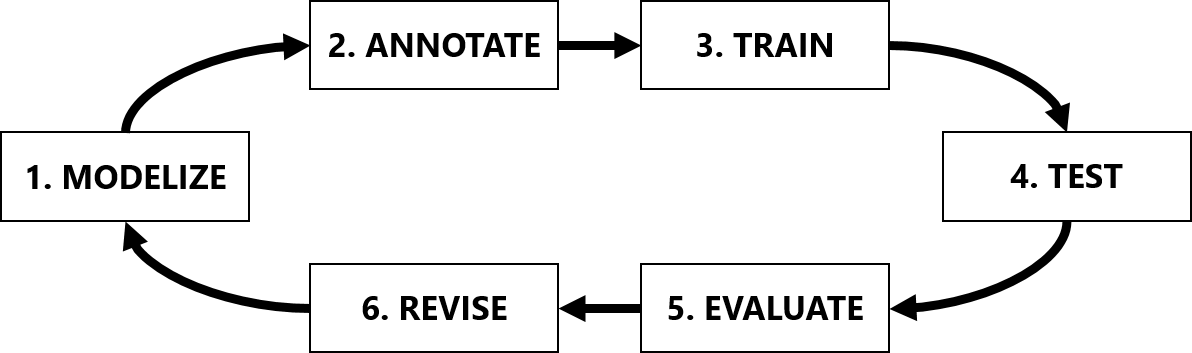
\includegraphics[width=0.95\textwidth]{figures/etatdelart-pustejovsky-2012-cycle-matter}
				\caption{
					Cycle \texttt{MATTER} structurant un projet d'annotation en six étapes principales: \textit{\textbf{M}odelize}, \textit{\textbf{A}nnotate}, \textit{\textbf{T}rain}, \textit{\textbf{T}est}, \textit{\textbf{E}valuate} et \textit{\textbf{R}evise}.
				}
				\label{figure:2.2.1-ORGANISATION-ANNOTATION-ETAPES-CLES-MATTER}
			\end{figure}
			
			% Collecte
			% M, A, mais aussi MAMA
			% TT, mais aussi Train Dev Test, puis Evaluate
			% Revise
			
			% Step 1: Modelisation
			\paragraph{1. Modelize.}
				\todo[inline]{SECTION: À RÉDIGER}
			
			% Step 2: Annotate
			\paragraph{2. Annotate.}
				\todo[inline]{SECTION: À RÉDIGER}
			
			% Step 3: Train
			\paragraph{3. Train.}
				\todo[inline]{SECTION: À RÉDIGER}
			
			% Step 4: Test
			\paragraph{4. Test.}
				\todo[inline]{SECTION: À RÉDIGER}
			
			% Step 5: Evaluate
			\paragraph{5. Evaluate.}
				\todo[inline]{SECTION: À RÉDIGER}
			
			% Step 6: Revise
			\paragraph{6. Revise.}
				\todo[inline]{SECTION: À RÉDIGER}
		
		
		%%%
		%%% Subsection 2.2.2: Portraits des acteurs intervenant sur un projet d'annotation.
		%%%
		\subsection{Portraits des acteurs intervenant sur un projet d'annotation}
		\label{section:2.2.2-ORGANISATION-ANNOTATION-ACTEURS}
			\todo[inline]{SECTION: À RÉDIGER: \\
				- Acteurs: Objectifs, Rôles, Compétences, ... ; \\
				~~~~ - Axe métier (business expert) ; \\
				~~~~ - Axe technique (data scientist) ; \\
				~~~~ - Axe manipulation (data analyst) ; \\
				~~~~ - Axe projet (project leader) ;
			}
		
		
		%%%
		%%% Subsection 2.2.3: Exemples de logiciels utilisés pour annoter.
		%%%
		\subsection{Exemples de logiciels utilisés pour annoter}
		\label{section:2.2.3-ORGANISATION-ANNOTATION-LOGICIELS}
			\todo[inline]{SECTION: À RÉDIGER: \\
				- Outils: Liste, Avantages, Inconvénients, Fonctionnalités ;
				~~~~ - Excel
				~~~~ - prodigy
					% - Glozz [Widlöcher & Mathet, 2009] http://www.glozz.org/
					% - Callisto [Day et al., 2004]
					% - MMAX2 [Müller, 2006] https://github.com/ottiram/MMAX2
					% - PALinkA [Orăsan, 2003]
					% - Gate [Cunningham_2022] https://gate.ac.uk/
					% - Brat [Stenetorp et al., 2012] http://brat.nlplab.org/
					% - WebAnno [Yimam et al., 2013] https://webanno.github.io/webanno/
					% - Inception [Klie et al., 2018] https://inception-project.github.io/
			}
		
		
		% Conclusion.
		\begin{leftBarSummary}
			\begin{todolist}
				\item[\itemok] Un projet d'annotation s'organise généralement en cycle (\texttt{MATTER}) au cours duquel l'annotateur créé une représentation mentale des données, réalise son annotation, entraîne son modèle, puis révise sa représentation mentale des données en fonction des performances du modèle obtenu.
				\item[\itemok] Un tel projet d'annotation nécessite une diversité de connaissances et de compétences (\textit{connaissances métiers, connaissances techniques, maîtrise de l'apprentissage automatique, ...}), faisant ainsi collaborer un grand nombre d'acteurs qualifiés pour une ou plusieurs phase du cycle d'annotation.
			\end{todolist}
		\end{leftBarSummary}
	
	
    %%%%%--------------------------------------------------------------------
    %%%%% Section 2.3: Les nombreux défis de l'annotation
    %%%%%--------------------------------------------------------------------
    \section{Les nombreux défis de l'annotation}
	\label{section:2.3-DEFIS-ANNOTATION}
		\todo[inline]{SECTION: TITRE À TROUVER: "\textit{Défis annotation}"}
		\todo[inline]{SECTION: À RÉDIGER: \\
			- Les données doivent être représentatives (Qualité, Biais, Equilibrage, ...) ; \\
			- Donc la tâche est complexe (...) ; \\
			- Donc les opérateurs régulent leur charge de travail () !
		}
		
		
		%%%
		%%% Subsection 2.3.1: Défis concernant le besoin de qualité des données.
		%%%
		\subsection{Défis concernant le problème de qualité des données}
		\label{section:2.3.1-DEFIS-ANNOTATION-ASPECT-DONNEES}
			\todo[inline]{SECTION: TITRE À TROUVER: "\textit{Données de qualité}"}
			\todo[inline]{SECTION: À RÉDIGER}
		
		
		%%%
		%%% Subsection 2.3.2: Défis concernant la complexité inhérente à la tâche d'annotation.
		%%%
		\subsection{Défis concernant la complexité inhérente à la tâche d'annotation}
		\label{section:2.3.2-DEFIS-ANNOTATION-ASPECT-COMPLEXITE}
			\todo[inline]{SECTION: TITRE À TROUVER: "\textit{Tache complexe}"}
			\todo[inline]{SECTION: À RÉDIGER}
		
		
		%%%
		%%% Subsection 2.3.3: Défis concernant les différences de comportements intra- et inter-annotateurs.
		%%%
		\subsection{Défis concernant les différences de comportements intra- et inter-annotateurs}
		\label{section:2.3.3-DEFIS-ANNOTATION-ASPECT-HUMAIN}
			\todo[inline]{SECTION: TITRE À TROUVER: "\textit{Régulation de la charge de travail}"}
			\todo[inline]{SECTION: À RÉDIGER}
		
		
		% Conclusion.
		\begin{leftBarSummary}
			\begin{todolist}
				\item[\itemok] L'enjeu d'un projet d'annotation consiste à avoir des données de qualité qui soient représentatives du problème à traiter ;
				\item[\itemok] Or la tâche d'annotation et son exigence de qualité engendre de la complexité, et donc une charge de travail élevée ;
				\item[\itemok] Pour réguler cette charge de travail élevée, chaque opérateur va adapter sa tâche pour la rendre supportable, créant ainsi des différences de comportement.
			\end{todolist}
		\end{leftBarSummary}
	
	
    %%%%%--------------------------------------------------------------------
    %%%%% Section 2.4:
    %%%%%--------------------------------------------------------------------
    \section{Techniques et organisations avancées d'annotation}
	\label{section:2.4-AVANCEES-ANNOTATION}
		\todo[inline]{SECTION: TITRE À TROUVER: "\textit{Techniques avancées d'annotation}"}
		\todo[inline]{SECTION: À RÉDIGER: \\
			- Sur les données: ... \\
			- Sur la complexité: ... \\
			- Sur les annotateurs: ...
		}
		
		
		%%%
		%%% Subsection 2.4.1: Avancées concernant le besoin de qualité des données.
		%%%
		\subsection{Avancées concernant le besoin de qualité des données}
		\label{section:2.4.1-AVANCEES-ANNOTATION-ASPECT-DONNEES}
			\todo[inline]{SECTION: TITRE À TROUVER: "\textit{Données de qualité}"}
			\todo[inline]{SECTION: À RÉDIGER}
		
		
		%%%
		%%% Subsection 2.4.2: Avancées cla diminution de la complexité de la tâche d'annotation
		%%%
		\subsection{Avancées concernant la diminution de la complexité de la tâche d'annotation}
		\label{section:2.4.2-AVANCEES-ANNOTATION-ASPECT-COMPLEXITE}
			\todo[inline]{SECTION: TITRE À TROUVER: "\textit{Tache complexe}"}
			\todo[inline]{SECTION: À RÉDIGER}
		
		
		%%%
		%%% Subsection 2.4.3: Concernant la réduction des différences de comportements intra- et inter-annotateurs.
		%%%
		\subsection{Avancées concernant la réduction des différences de comportements intra- et inter-annotateurs}
		\label{section:2.4.3-AVANCEES-ANNOTATION-ASPECT-HUMAIN}
			\todo[inline]{SECTION: TITRE À TROUVER: "\textit{Régulation de la charge de travail}"}
			\todo[inline]{SECTION: À RÉDIGER}
		
		
		% Conclusion.
		\begin{leftBarSummary}
			\begin{todolist}
				\item[\itemok] (TODO)
			\end{todolist}
		\end{leftBarSummary}

    %%%%%--------------------------------------------------------------------
    %%%%% Section 2.5:
    %%%%%--------------------------------------------------------------------
    \section{(\textit{conception toujours difficile en entreprise})}
	\label{section:2.5-RETOUR-EXPERIENCES-INDUSTRIELLES}
		\todo[inline]{SECTION: TITRE À TROUVER: "\textit{REX entreprise}"}
		\todo[inline]{SECTION: À RÉDIGER: \\
			- Modélisation toujours compliquée ; \\
			- Expert métier "pas à leur place" ; \\
			- Peu de stratégies de notre revue mises en oeuvre...
		}